% Chapter 1

\chapter{Introduction} % Chapter title

\label{ch:introduction} % For referencing the chapter elsewhere, use \autoref{ch:introduction} 

%----------------------------------------------------------------------------------------

National statistical offices disseminate official statistics in statbanks where it is available to citizens and institutions via web interfaces.
 
All the statistical offices in the Nordic region and in several other countries around the world use an installation of the statbank application, PxWeb, to disseminate official statistics.
 
PxWeb is lead by Statistics Sweden and developed in cooperation with other national statistical offices, among them Statistics Norway and Statistics Finland.

\section{Statement of the Problem}
User research performed in the Faroe Islands shows that many of the mediocre and novice users have a difficult time using the PxWeb interface. Similar findings have been found by other statistical offices, which are using the PxWeb statbank application. This is therefore a cross-national problem since users in several countries using PxWeb are facing the same usability issues.
 
One of the main challenges for the users across different sectors is to find the right data in the statbank. The user interaction tends to involve many clicks to get data and when the data finally is returned from the application it often is not what user is expecting. This often results in users giving up in finding the right data.
 
The user journey in the statbank starts by navigating the folder structure and then finding the right table\ref{fig:List}. When the user has found a relevant table the user has to choose multiple categories from several statistical variables\ref{fig:selectors} and then click the submit button to display the data\ref{fig:selectors}. If the data is not what the user is expecting the user has to go over this procedure once again.




\begin{figure}[bth]
    \myfloatalign
    \subfloat[List]    
    {\label{fig:List}
    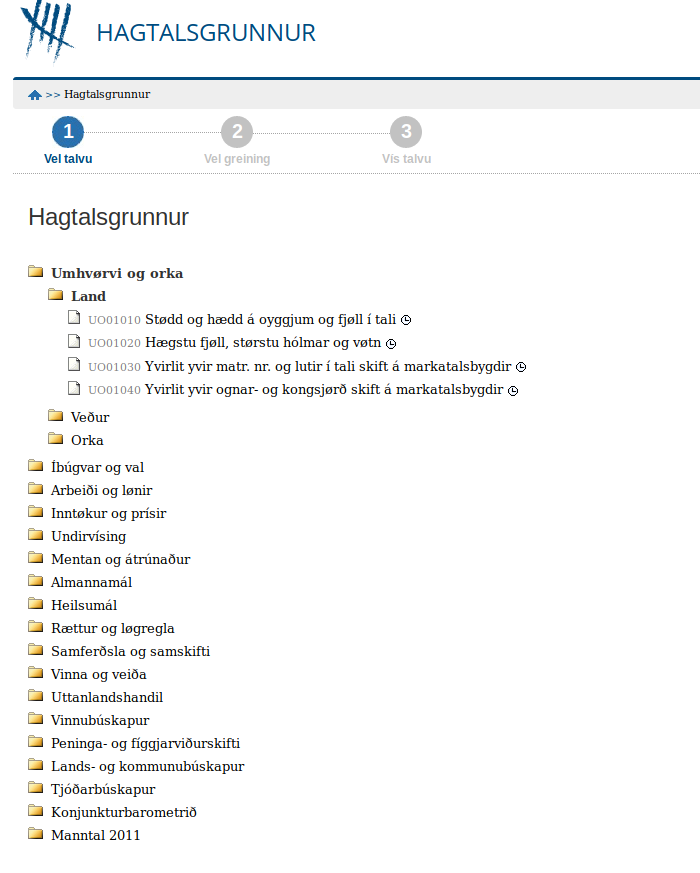
\includegraphics[width=.3\linewidth]{gfx/ui1.png}}
    \subfloat[Selectors]
    {\label{fig:selectors}
    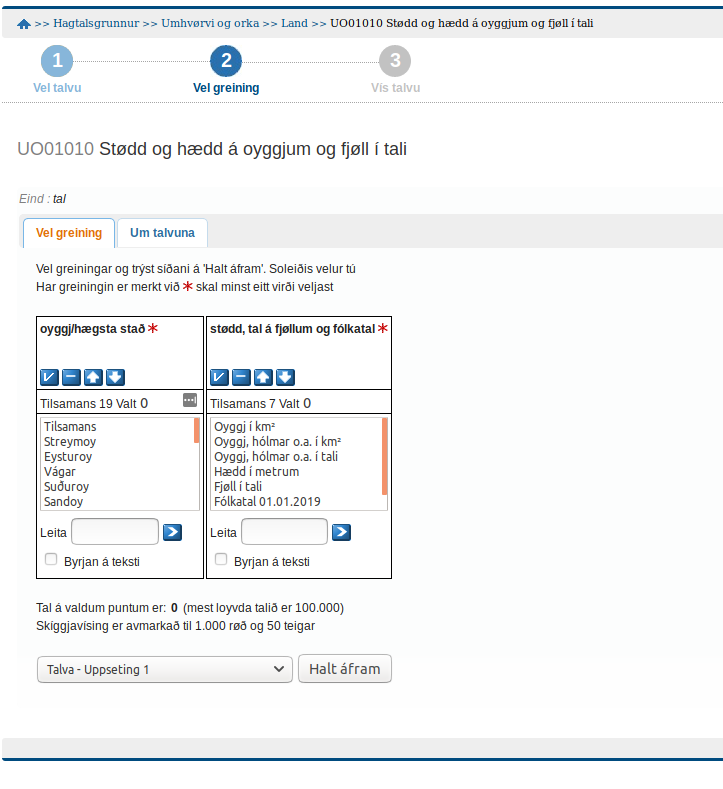
\includegraphics[width=.3\linewidth]{gfx/ui2.png}} 
    \subfloat[Result]
    {\label{fig:result}
    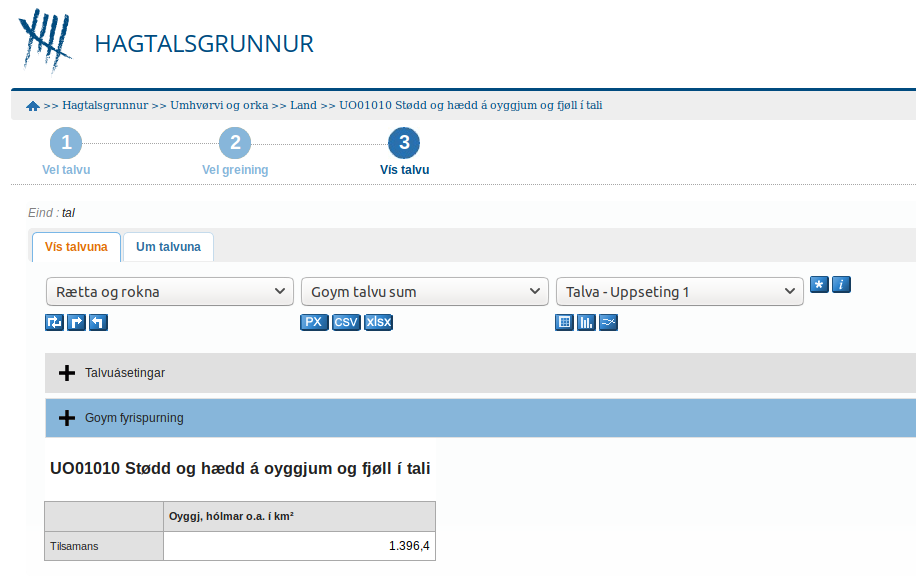
\includegraphics[width=.3\linewidth]{gfx/ui3.png}}   
    \end{figure}
In ISO 9241\footnote{\href{https://www.iso.org/search.html?q=ISO\%209241}{ISO 9241}\label{iso9241}} usability is defined as the effectiveness, efficiency and satisfaction with which specified users achieve specified goals in particular environments. In this case this means users finding the right data in the statbank.
 
Effectiveness is the accuracy and completeness with which the users can achieve specified data in PxWeb.  Efficiency is the resources expended such as time or number of clicks in relation to the accuracy and completeness of getting the right data. Satisfaction is the comfort and acceptability of the work system to its users and other people affected by its use.

From a usability perspective it seems that there is a lack of effectiveness and efficiency in the PxWeb application. This requires a new approach to get and display the data from the statbank application.

\section{Significance of the Study}
In this thesis I am aiming to improve the effectiveness and efficiency of the application by developing a prototype of a new web interface that exploits and utilizes the API in the PxWeb statbank. I aim to establish a direct communication between interface and the API in order to get data, manipulate data and displaying data instantly.

In this approach the user will instantly be shown data when the user has chosen a category from a statistical variable. This differs significantly from current approach where the user has to choose multiple categories in several statistical variables and then click the submit button to get the data. 

This new approach reduces the number of clicks and the time used to get data significantly.

It will make user interface more intuitive and easier to use.
 
\section{Addressing the Problem}
The problem will be address by using the right technology and the software engineering approach such as the software methodology\footnote{A software methodology is a set of related activities that leads to the production of software} Agile and the five framework activities:

\begin{itemize}
    \item Communication
    \item Planning
    \item Modeling
    \item Construction
    \item Deployment
\end{itemize}